\documentclass{article}

\usepackage[utf8]{inputenc}
\usepackage{amsfonts}
\usepackage{todonotes}
\usepackage{cryptocode}
\usepackage{algorithm,algorithmic}

\newcommand{\adv}{{\sf Adv}}
\newcommand{\madv}{\mathsf{Adv}}

\title{Encrypted SNI}
\author{No Name}
\date{\today}

\begin{document}

\maketitle

\section{Introduction}

In this note we try to capture the privacy guarantees of Encrypted SNI \cite{ietf-tls-esni-04}.

%% XXX: describe encrypted SNI properties (relate to tunneling), and describe known
% attacks against existing designs.
%% XXX: notation
%% XXX: security model, including binding requirements
%% XXX: ESNI tunnel-based design (with full key schedule) and wrapping logic
%% XXX: security analysis

\section{Notation}

\todo[inline]{NOTE(caw): Forgive me for such abusive notation!}

TLS is an authenticated key exchange protocol composed of sub-protocols. Importantly, TLS has
a handshake and record protocol. The handshake protocol uses handshake messages to perform
key exchange and its many facets, including, among other things, cryptographic algorithm
selection and peer authentication. Let $h \in \{0,1\}^{2^{16}}$ be a handshake message 
composed of arbitrary data, and let $\mathbf{H}$ be the set of possible handshake messages.

The record protocol uses messages with headers consisting 
of type, length, and version to send data between peers. This data is either a plaintext 
handshake message or encrypted blob. For our analysis, let $r = (d, p)$ be a 
record composed of direction $d \in \{0,1\}$ and payload $p \in \{0,1\}^{2^{16}}$. Let
$\mathbf{R}$ be the set of all possible records. Let $\mathbf{P} = \{0,1\}^{2^{16}}$ 
be the set of possible payloads. Note, by definition $\mathbf{H} \subset \mathbf{P}$.
Let $\mathsf{Message}$ be a function that returns the plaintext message for a given
record $r$, or nothing if the record is encrypted.

We model a TLS handshake as a trace of records and their metadata sent between a client and server. 
(Metadata may include, among other things, record lengths as observed on the wire.) 
Formally, let $\vec{t} = <r_0, r_1, \dots, r_n\>$ be a trace of $n$ records, where 
$r_i = (d_i, p_i) \in \mathbf{R}$. Let $\mathbf{T}$ be a set of traces. 

Without loss of generality, in TLS 1.3, there are three types of messages observed
on the wire: ClientHello (CH), ServerHello (SH), and ApplicationData (AD). Let $\mathbf{CH}$ 
and $\mathbf{SH}$ be the set of possible CH and SH handshake messages generated by 
clients and servers, respectively. Each CH, SH, and AD message belongs to $\mathbf{P}$.

Let $N \in \{0,1\}^{2^{16} - 1}$ be a name, and let $\mathbf{N}$ be the set of names. 
CH messages typically carry names as one of their parameters.

Let $\mathsf{ClientConfig}$ be a set of parameters that determine a client's configuration,
including supported ciphersuites, named groups, extensions, etc. 
Let $\mathbf{CC}$ be the set of all client configuration parameters.
Similarly, let $\mathsf{ServerConfig}$ be a set of parameters that determine a server's configuration,
and let $\mathbf{SC}$ be the set of all client configuration parameters.
Clients produce CH messages to a given server, identified by its name $N$, and configuration
$\mathsf{ClientConfig}$, using a function $\mathsf{GenerateCH}: \mathbf{N} \times \mathbf{CC}$.
Servers produce SH messages (and do other parameter selection) based on a CH message and 
server configuration, using a function $\mathsf{GenerateSH}: \mathbf{CH} \times \mathbf{SC}$.

The function $\mathsf{Metadata}$ takes as input a CH or SH and returns the set of metadata,
or parameters, associated with the message, including the server name $N$, ciphersuite list,
named groups, and other extensions that are visible on the wire. The function
$\mathsf{PublicMetadata}$ returns the same output as $\mathsf{Metadata}$, except that
the server name is omitted. 

Using the notation above, every handshake is a probabilistic function of some server name $N$,
$\mathsf{ClientConfig}$, and $\mathsf{ServerConfig}$. In particular:
%
\begin{itemize}
    \item A client generates a CH message using $N$ and $\mathsf{ClientConfig}$.
    \item The recipient server generates a SH message using the input CH and $\mathsf{ServerConfig}$.
    \item The remainder of the handshake contains encrypted AD messages.
\end{itemize}
%
Thus, let $\mathsf{Handshake}$ be a function that takes as input $N$,
$cc = \mathsf{ClientConfig}$, and $sc = \mathsf{ServerConfig}$ and produces a trace 
$t = r_1, r_2, r_3, \dots$, where $\mathsf{Message}(r_1)$ is a CH and 
$\mathsf{Message}(r_2)$ is a SH. Let $\mathsf{PublicHandshake}$ be a similar
function that computes $t = r_1, r_2, r_3, \dots = \mathsf{Handshake}(t, cc, sc)$ and returns 
$t^v \mathsf{PublicMetadata}(r_1), \mathsf{PublicMetadata}(r_2), r_3, \dots$. That is,
it returns publicly visible metadata associated from a handshake trace. 

Finally, we define a function $\mathsf{SNI}$ which takes as input a handshake trace $t$
and returns the name $N$ which was used to generate $t$. 


% Let $N_i$ be the SNI value in ClientHello $h^c_i$, where $N_i \in \mathbf{N} = \{0,1\}^{2^{16} - 1}$.
% Let $H(N_i)$ be a \emph{handshake trace} comprised of ClientHello $h^c_i$ with SNI $N_i$, ServerHello $h^s_i$,
% and message trace $\vec{t}$, i.e., $H(N_i) = (h^c_i, h^s_i, \vec{t})$. Let $\mathbf{H}$ be the set of possible
% handshake traces. Let $\mathsf{SNI}$ be a function that takes as input a handshake trace $H \in \mathbf{H}$ 
% and returns the SNI name $N_i$ inside the ClientHello.

% Let $\mathsf{config}_s$ be the set of statically configured parameters for a server. These parameters
% might include, for example, supported ciphersuites and certificates. Similarly, let $\mathsf{config}_c$
% be the set of statically configured paramaeters for a client. These might include the set of supported
% ciphersuites, among other things. Let $\mathsf{params}_c$ be a
% similar set of (publicly visibile) parameters associated with a ClientHello $h^c_i \in \mathbf{CH}$, modulo
% $\mathsf{SNI}(h^c)$. Let $\mathsf{ClientParams}$ be a function which takes as input a ClientHello 
% $h^c_i \in \mathbf{CH}$ and returns $\mathsf{params}_c$. Similarly, let $\mathsf{params}_s$ be the
% parameters associated with a ServerHello. Let $\mathsf{ServerParams}$ be a function which takes as 
% input a ServerHello $h^s_i \in \mathbf{SH}$ and returns $\mathsf{params}_s$. Given a handshake 
% $H(N_i) = (h^c_i, h^s_i, \vec{t})$, the publicly visible metadata for this handshake is given as 
% $H^v(N_i) = (\mathsf{ClientParams}(h^c_i), \mathsf{ServerParams}(h^s_i), \vec{t}$.

% We also define a function $\mathsf{Select}$ which takes as input a ClientHello $h^c_i \in \mathbf{CH}$ and
% parameters structure $\mathsf{config}$ and produces a ServerHello $h^s_i \in \mathbf{SH}$. Specifically,
% $h^s_i = \mathsf{Select}(h^c_i, \mathsf{config})$.

\section{Security Model}

In this section, we describe two variants of an ESNI adversary: passive and active.

\subsection{Passive Adversary}

We base our definition of privacy on the indistinguishability of handshake traces. At a high level, 
this means the following. Assume there are two handshake traces $t_0$ and $t_1$, and an adversary \adv\
sees the publicly visibile metadata for these traces, i.e., $p_0^v$ and $p_1^v$. We say that the 
handshake traces are \emph{SNI-agnostic} if \adv\ cannot determine if $\mathsf{SNI}(t_0) = \mathsf{SNI}(t_1)$.
Roughly speaking, a handshake is SNI-agnostic if the set of publicly visible metadata 
associated with a handshake \emph{does not vary} based on SNI, which therefore 
implies that the SNI leaks no information about the handshake traces.

\begin{figure}
    \centering
    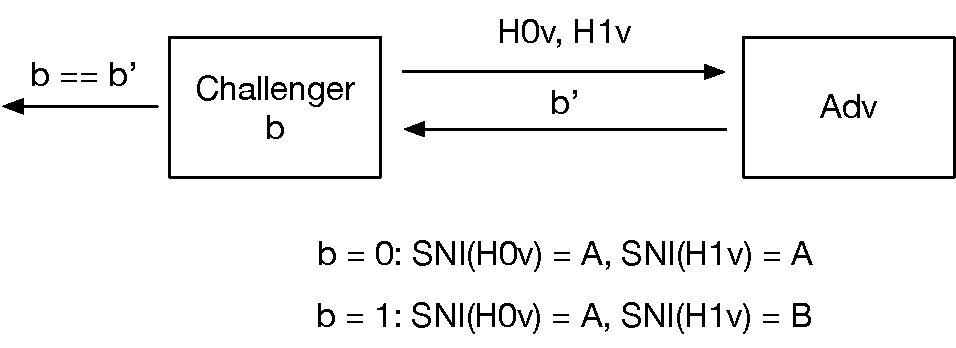
\includegraphics[scale=0.7]{esni_game_passive.pdf}
    \caption{Passive ESNI Privacy game}
    \label{fig:passive-game}
\end{figure}

We capture this definition in the following {\sf NameGame}, which is defined in Algorithm \ref{alg:esnigame}.

\begin{algorithm}
\caption{{\sf NameGame}} 
\label{alg:esnigame}
\begin{algorithmic}[1]
%   \scriptsize
  \STATE On input security parameter $\lambda$, $\mathbf{N}$, $\mathbf{CC}$, $\mathbf{SC}$, and adversary \adv\, a challenger $C$ initializes \adv\ with $\mathbf{CC}$, $\mathbf{SC}$, 
  and $\mathsf{N}$. 
  \STATE $C$ chooses a random bit $b$. If $b = 0$, $C$ gives produces a challenge tuple
  $(\mathsf{PublicHandshake(N_0)}, \mathsf{PublicHandshake(N_1)}$, where 
  $N_0,N_1 \gets \mathbf{N}$ and $N_0 \not= N_1$.
  Otherwise, $C$ produces challenge tuple 
  $(\mathsf{PublicHandshake(N_0)}, \mathsf{PublicHandshake(N_1)}$, where 
  $N_0,N_1 \gets \mathbf{N}$ and $N_0 = N_1$.
  \STATE \adv\ replies with a bit $b'$.
  \STATE Output $1$ if $b = b'$, otherwise output $0$.
\end{algorithmic}
\end{algorithm}

We say that \adv\ wins $\mathsf{NameGame}$ if it outputs $1$, i.e., if \adv\ was able to determine distinguish 
two handshakes using the same ESNI (or not). We define the advantage \adv\ has in this game as
$|\Pr[\mathsf{ESNIGame}(\lambda, \mathbf{N}, \mathsf{config}, \madv)] - \frac{1}{2}|$. That is, 
the probability that \adv\ guesses $b$ correctly less the probability that it guesses incorrectly. 

We say that a handshake trace is \emph{SNI agnostic} if, for all PPT adversaries \adv, \adv's advantage in 
winning $\mathsf{ESNIGame}$ is negligibly small in $\lambda$. 

%%% Required property:
% - All input to the server [ClientParams()] is bound to ESNI // In the active case, adversary can take output of ClientHelloGen and produce its own CH, which is input to the server.
% - All output produced by the seraver [ServerParams()] is bound to the ESNI

\subsection{Active Adversary}

An active adversary has the ability to generate handshake traces at will. We assume servers are neither malicious nor compromised. 
Therefore, adapting our model for privacy requires extending $\mathsf{ESNIGame}$ to give \adv\ an oracle for producing handshake
traces with an SNI of its choosing. We define this oracle as $\mathcal{O}_H$, and it takes as input an SNI $N \in \mathbf{N}$
and returns a handshake trace $H(N) \in \mathbf{H}$. The modified game, called $\mathsf{ActiveESNIGame}$, proceeds as follows:

\begin{algorithm}
\caption{{\sf ActiveESNIGame}} 
\label{alg:active-esnigame}
\begin{algorithmic}[1]
%   \scriptsize
  \STATE On input security parameter $\lambda$, $\mathbf{N}$, $\mathsf{config}$, and adversary \adv\, a challenger $C$ initializes \adv\ with $\mathsf{config}$, $\mathsf{N}$, and access to $\mathcal{O}_H$.
  \STATE \adv\ queries $\mathcal{O}_H$ with SNI values of its choosing from $\mathbf{N}$ at most $\mathsf{poly}(\lambda)$ times.
  \STATE $C$ chooses a random bit $b$. If $b = 0$, $C$ gives produces a challenge tuple $(H^v(N_0), H^v(N_1))$, where $N_0,N_1 \in \mathbf{N}$ and $N_0 \not= N_1$, and where $H^v(N_0) = (\mathsf{ClientParams}(h^c_0), \mathsf{ServerParams}(\mathsf{Select}(h^c_0, \mathsf{config})), \vec{t})$.
  Otherwise, $C$ produces challenge tuple $(H^v(N_0), H^v(N_1)$, where $N_0,N_1 \in \mathbf{N}$ and $N_0 \not= N_1$, and both handshake traces are generated as in the other case.
  \STATE \adv\ continues querying $\mathcal{O}_H$ at most $\mathsf{poly}(\lambda)$ times.
  \STATE \adv\ replies with a bit $b'$.
  \STATE Output $1$ if $b = b'$, otherwise output $0$.
\end{algorithmic}
\end{algorithm}

%% TODO(caw): do we extend adv's capabilities to include those of the CK model for key exchange security? we probably do
% need to include this, as we don't want the ESNI mechanism to interfere with the secrecy of the session keys.

As before, we say that \adv\ wins $\mathsf{ActiveESNIGame}$ if it outputs $1$. We define the advantage \adv\ has in this game as
$|\Pr[\mathsf{ActiveESNIGame}(\lambda, \mathbf{N}, \mathsf{config}, \madv)] - \frac{1}{2}|$. And we say that a handshake trace
is \emph{SNI agnostic} with respect to an active attacker if \adv's advantage in winning $\mathsf{ActiveESNIGame}$ is negligibly 
small in $\lambda$.

\section{Session Ticket Oracle Attack}

Assume a server includes the negotiated SNI value inside
a resumption ticket. Moreover, assume that, upon receiving a ClientHello with a ticket
carrying an SNI, said server will also check that the SNI value in the ticket matches 
that of the negotiated SNI (from plaintext SNI or an ESNI extension). Upon mismatch, the
server aborts the connection, and upon success proceeds with the connection. 

This lets \adv\ use the ticket check as an oracle to determine if a candidate ClientHello
carrying an ESNI extension matches a ticket of the \adv's choosing. The attack works as follows.
First, \adv\ connects to a server using the SNI of its choosing and receives a ticket. Then,
\adv\ observes a ClientHello with ESNI sent to the same server. \adv\ uses its ticket with 
the same ClientHello contents to compute a binder and produce a modified ClientHello, which
is then forwarded to the server. If the server accepts the ticket, then \adv\ knows that the
SNI which it chose when fetching its ticket matches that of the client's ESNI extension. 

This oracle is possible because the full ClientHello and its ESNI contents are not atomically
bound to the resumption PSK. In particular, since the resumption PSK is not encrypted for the
same parties which can decrypt the ESNI, then this type of oracle will always be possible. 
Put differently, if attacker-controlled information can influence the handshake flow for an 
unknown ESNI, then this type of attack exists.

%%% idea: if ESNI encryption is IND-CPA-secure and cannot be modified, then handshake flow
% information is determined solely by the contents of that payload

\todo[inline]{Show this type of attack trace}

This implies that the ESNI encryption key must cover the resumption ticket. Consequently, 
since the resumption PSK covers the entire ClientHello, the ESNI key must cover the entire
ClientHello.

\todo[inline]{Does this imply that the ESNI MUST be bound to the PSK that's used? Either by making ESNI a PSK, or by tunneling the "real" CH with a PSK.}

\section{Re-Encryption Attacks}

Assume we go with the CH transformation described by Kazhuo et al., wherein the server makes a determination
to use the pre- or post-transformed CH for the transcript. This lets a malicious server do the following. 
Upon receipt of a transformed ClientHello, the server decrypts the ESNI value, and then forwards the pre-transformed
CH to backend server, which then completes the handshake with the pre-transformed CH in the transcript.

% XXX: this design only allows the handshake to be completed with the pre- or post-transformed CH. The pre-transformed
% CH has the "public" information, and the post-transformed CH has "private" information. A malicious server could take
% a pre-transforemd CH, apply its own transformation (on the same input CH) and send it to another server, who then
% thinks it came from the client. This wouldn't show up in the transcript if ESNI was negotiated, since only one of the 
% CHs was used (pre- if ESNI was negotiated, and post- if ESNI was not negotiated).

% Q: is this a problem? unsure, but it feels wrong for parties in the middle to be able to tamper with TLS messages
% arbitrarily without being noticed.

% XXX: this means the encryption context *must* be included in the transcript. Client-facing servers which can decrypt
% SNI process this just fine. Backend servers need to be given ESNI secrets via some other mechanism in order to process the SNI.

\bibliography{references}

\end{document}
